\documentclass[]{article}
\usepackage{amsmath}
\usepackage{graphicx}
\usepackage{caption}
\usepackage{mathtools}
\usepackage{cleveref}
\usepackage{courier}
\usepackage{subcaption}
\usepackage{units}
\usepackage{float}
\usepackage{placeins}
\usepackage{needspace}
\usepackage{amssymb}
\usepackage[margin=1in]{geometry}
\graphicspath{{/home/john/Documents/Python/Networks/figures/} }
%opening

\title{Network Project}
\author{John Norrie}

\begin{document}

\maketitle

\begin{abstract}
Networks are an important modelling tool in many fields of science and social science. From modelling the internet to the spread of epidemics, networks provide an intuitive and ... approach to concepts so popularity and contact. \\
In this paper will be presented theoretical and numerical analysis of three separate models. The first is a Barabasi Albert Model. This model uses preferential attachment based on the degree size. The second is concerned with random attachment, and the third uses the concept of random walks on the graph to determine which nodes are used in attachment.\\
There are two key areas which will be analysed in detail; the first of which is the degree probability distribution, and the second is the highest recorded degree. In both of these areas, theoretical derivations will be provided, and supported or criticised using numerical data.  
\end{abstract}
\clearpage
\section{Implementation of the BA Model}
The Barabasi Albert model(BA) is alogirthm used to create freescale networks which rely on preferential attachment when adding new nodes. This means that nodes with a high degree are more likely to be attached to be new nodes. The algorithm works as follows:
\begin{enumerate}
	\item Create an initial graph, $\mathcal{G}_0$ at $t_0$ 
	\item Increment $t \rightarrow t+1$
	\item Add one new vertex
	\item Add $m$ new edges from the new vertex to vertices in the network, each with a probability of attachment $\Pi \propto k$ where $k$ is the degree of each vertex.
	\item Repeat from step 2 until the network contains $N$ vertices.
\end{enumerate}



The biggest factors when implementing this model is speed. The size of the networks we wish to analyse mean that a fast program is essential. The programme I developed creates a list of numbers, each couplet defining an edge. At the $k^{th}$ time step, a number is chosen at random (uniformly distributed) from this sequnce (x). then the number k and x are appended to the end of the list. This is carried out for $N$ time steps, after which the frequency of numbers are counted, and the outcome is the degree of each node. An example is shown below. \\
\begin{enumerate}
\item -$G=[0,1,0,2,1,2]$ is our starting graph, $N=3$, $m=3$
\item Add 2 new edges
\item 0 and 2 chossen randomly
\item $\Rightarrow G=[0,1,0,2,1,2,3,0,3,2]$
\item \text{Ending the iteration the counts are sorted, giving degree distribution:}\\ $deg(G)=[3,2,3,1]$
\end{enumerate}
This forces prereferntial attachement on the system, as if number $i<k$ appears more times in the sequence(e.i has more egdes attached), it is more likely to be chosen.
\subsection{Initial Graph}
There are a few points of ambiguity in this model. The first of which is with respect to $\mathcal{G}_0$. There is no explicit guidance on how to choose $\mathcal{G}_0\!$, however the choice of starting graph does have an affect. When deriving the master equation for the network, we will use the approximation that $E(t)=mN(t)$ (where $E(t)$ and $N(t)$ are the number of edges and nodes in the graph at time $t$ respectively.) for larger $t$. However we can make this approximation exact by choosing an $\mathcal{G}_0$ such that $E(0)=mN(0)$.\\
There are many graphs that satisfy this relation, however I would like the starting graph to be as small as possible. Doing this reduces the influence at has on the actual model. Therefore I used a complete graph. \\
The number of edges in a complete graph is,
\begin{equation}
E=\sum_{n=1}^{N} n-1 = \frac{N(N-1)}{2}
\end{equation}
Therefore, applying the conditon, 
\begin{align}
E(0)=mN(0) &\Rightarrow \frac{N(0)(N(0)-1)}{2}=mN(0)\\
&\Rightarrow N(0)^2 - (2m +1)N = 0\\
&\Rightarrow N=0  \text{(trivial)   and} \quad N=2m+1
\end{align}
Therefore choosing $\mathcal{G}_0$ to be a complete graph with $2m+1$ nodes is sufficient for the condition $E(0)=mN(0)$.
\begin{figure}[htp]
	\centering
	%\includegraphics{figure_1.png}
	
	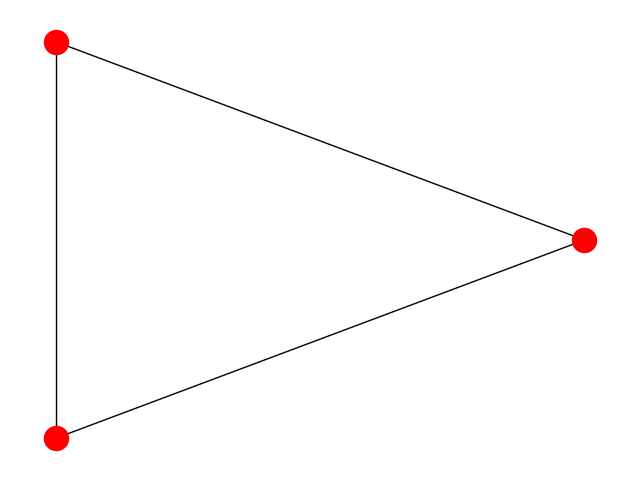
\includegraphics[width=.3\textwidth]{G0m=1.png}\hfill
	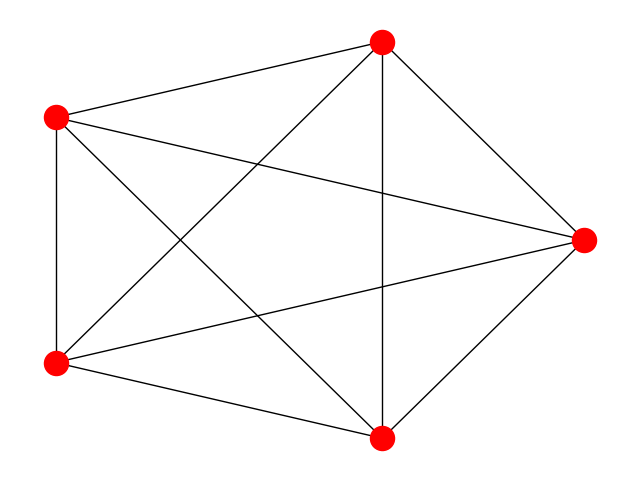
\includegraphics[width=.3\textwidth]{G0m=2.png}\hfill
	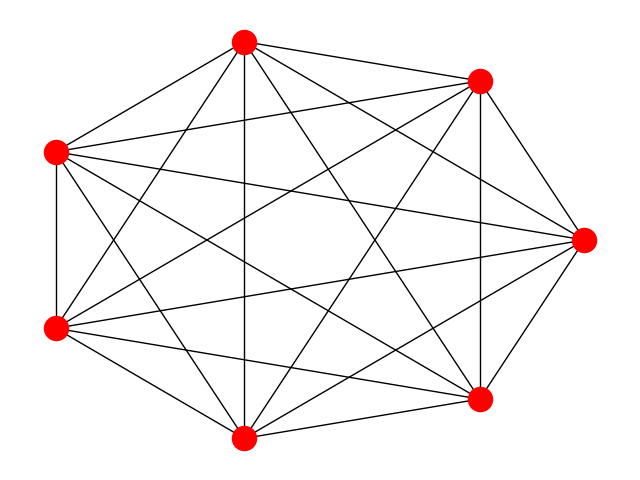
\includegraphics[width=.3\textwidth]{G0m=3.png}
	\caption{\textit{$\mathcal{G}_0$ for m=1,2,3 respectively.}}
\end{figure}
\subsection{Double Edges}
It is also uncear in this model whether we allow more than one edge connecting two nodes. How this might affect the outcome is uncertain. If there are nodes with large degree, according to preferential attachment, they are more likely to be choosen again when attaching more edges, so they may be very common. On th other hand, the probability of a node being chosen twice in a large network is very small, and so double edges may be very are.  In testing the latter case was proven to be correct(figure 2). Although this is compelling evidence, I decided to work with a model which excludeds double edges, as it is more applicable in physical interpretation. For example, when modelling the links between websites or friendships, double undirected edges are nonsensical. 
\begin{figure}[htp]
	\centering
	\includegraphics[width=.5\textwidth]{Edgey1.png}\hfill
	\includegraphics[width=.5\textwidth]{Edgey2.png}\hfill
	\caption{\textit{Degree distribution for m=10, N=1000 and N=100,000 respectively. There is little diference between between the distribution where double edges were allowed, and where double edges weren't allowed. }}
\end{figure}
\subsection{Testing}
A way to test whether the programme is working is to analyse the degree distribution(figure 3) so see whether it is what we would expect from a BA model.
\begin{figure}[H]
 	\makebox[\linewidth][c]{%
 		\begin{subfigure}{.6\textwidth}
 			\centering
 			\includegraphics[width=\textwidth]{Theoretical3.png}
 			\caption{}
 		\end{subfigure}%
 		\begin{subfigure}{.6\textwidth}
 			\centering 
 			\includegraphics[width=\textwidth]{Theoretical5.png}
 			\caption{}
 		\end{subfigure}
 	}
 	\caption{(a) shows the degree distributions of a single trial for $N=10^5$ and $m=1,2,3,4$. They exhibits many features of the BA model. Firstly there is a prominent 'fat tail' to our distribution. This relates to having single nodes with high degrees(hubs), however the majority having fairly low degree. \\
 	Secondly the figure shows that there distributions follow a powerlaw, $k^{-\gamma}$, where $\gamma$ will be derived later. This is a definition of a scale free network. \\
 	(b) shows the degree distributions of 1000 trails for $N=10^4$ and $m=1,2,3,4$. The fat tail of the distribution is a lot more defined, since there is more data. I shall use this method of rapeating trials throughout my report to obtain better statistics and understanding.}
\end{figure}

\section{Degree Distribution of the BA model}
\subsection{Theoretical Derviation}
There are a few ways of approximating the degree distribution $p(k)$, all of which use the master equation. The master equation of a system, desrcibes how the system changes with time evolution. When building the network, for the BA model the master equation is,
\begin{equation}
n(k,t+1)=n(k,t)+m\Pi(k-1,t)n(k-1,t)-m\Pi(k,t)n(k,t)+\delta_{k,m}
\end{equation}
Where $\Pi(k,t)$ is the probaility of an edge being attached to a particular node of degree $k$.
Since we are taking $\Pi(k,t) \propto k$, and that the probabilities are normalised, way get that:
\begin{equation}
\Pi(k,t)=\frac{k}{\sum_{k=1}^{\infty}{kn(k,t)}}
\end{equation}
Where $n(k,t)$ is the number of nodes of degree k. Also, each edge is reponsible for two degrees, so,
\begin{equation}
\Pi(k,t)=\frac{k}{2E(t)}
\end{equation}
I have already discussed that $E(t)=mN(t)$ using the initial conditions chosen, and so substituting $E(t)$ for $N(t)$, the probability becomes  $\Pi(k,t)=\frac{k}{2mN(t)}$. Applying this to (1):
\begin{equation}
n(k,t+1)=n(k,t)+\frac{(k-1)n(k-1,t)}{2N(t)}-\frac{kn(k,t)}{2N(t)}+\delta_{k,m}
\end{equation}
Now we define the probability of choosing any node of degree $k$ at time $t$: 
\begin{align}
&p(k,t)=\frac{n(k,t)}{N(t)}\\
(1) \Rightarrow \quad &N(t+1)p(k,t+1)-N(t)p(k,t)=\frac{(k-1)}{2}p(k-1,t)-\frac{k}{2}p(k,t)+ \delta_k,m
\end{align}
In order to go further, we assume that $p(k,t)$ converges for large $t$. That is that $p_{\infty}=lim_{t \rightarrow \infty} p(k,t)$\\Applying this to (6) the final form of our master equation becomes:
\begin{equation}
(N(t+1)-N(t))p_{\infty}(k)=-\frac{(k-1)}{2}p_{\infty}(k-1)-\frac{k}{2}p_{\infty}(k)+ \delta_k,m
\end{equation}
We note that $N(t)=t$  and so we find the final form of the master equation:
\begin{equation}
p_{\infty}(k)=\frac{1}{2}((k-1)p_{\infty}(k-1)-kp_{\infty}(k)) +\delta_{k,m}
\end{equation}
\subsection{Continuous Approximation}
Equation (12) can be used to find the degree distribution for the model.
An approximation of this distribution can be found the continuous case,$k+1 \rightarrow k + \Delta k$. (12) becomes:
\begin{equation}
{p(k) \approx \lim\limits_{\Delta k \rightarrow 0}\frac{-\frac{1}{2}((k-\Delta k )p_{\infty}(k-\Delta k)-kp_{\infty}(k)) +\delta_{k,m}}{\Delta k} }
\end{equation}
\begin{equation}
\Rightarrow p(k)\approx \frac{\partial kp_{\infty}(k)}{\partial k}
\end{equation}
By inspection we find that $p(k) \propto k^{-3}$ is a solution. This means that the degree distribution follows a power law, and so implies that the BA model is scale free. \\
As k grows the continous case becomes more accurate, as relatively the difference between $k$ and $k-1$ becomes less. So we would expect this case to be true as $m\rightarrow \infty$, as this forces higher degrees on the system. 
\subsection{Difference Derivation}
It is possible to derive a solution from the difference equation. First we look at $k>m$ and rearrange (7):
\begin{equation}
\frac{p_{\infty}(k)}{p_{\infty}(k-1)}=-\frac{k-1}{2(k+1)}
\end{equation}
We use an identity of the Gamma function. The equation:
\begin{equation}
\frac{f(z)}{f(z-1)}=\frac{z+a}{z+b}
\end{equation}
Has solution,
\begin{equation}
f(z)=A\frac{\Gamma(z+1+a)}{\Gamma(z+1+b)}
\end{equation}
Therefore our difference equation has solution
\begin{equation}
p_{\infty}(k)=A\frac{\Gamma(k)}{\Gamma(k+2)}
\end{equation}
Using the identity $\Gamma(n)=(n-1)!$ for $n \in \mathbf{N}_0$, the solution becomes:
\begin{equation}
p_{\infty}(k)=\frac{A}{k(k+1)(k+2)}
\end{equation}
The constant $A$ can be found by looking at the boundary case ($k=m$) of (7),
\begin{align}
&p_{\infty}(m)=-\frac{m}{2}p_{\infty}(m)+1\\
&\Rightarrow p_{\infty}(m)=\frac{1}{m+2}
\end{align}
This boundary conditon implies that, 
\begin{equation}
A= 2m(m+1)
\end{equation}
Thus we derive the solution to the difference equation as:
\begin{equation}
p_{\infty}(k)=\frac{2m(m+1)}{k(k+1)(k+2)}
\end{equation}
I expect this distribution to be more accurate than that obtain by the continuous derivation, as I have made less assumptions and approximations.\\
Checking that this equation is normalised,
\begin{align*}
&\sum_{k=0}^{\infty} p_{\infty}(k)=2m(m+1)\left\{ \sum_{k=0}^{\infty}\frac{1}{k(k+1)(k+2)}\right\}\\
&\Rightarrow = 2m(m+1)\left\{\sum_{k=0}^{\infty} \frac{1}{2k} - \frac{1}{k+1} + \frac{1}{2(k+2)} \right\}\\
&\Rightarrow = 2m(m+1)\left\{\frac{1}{2}\left(\sum_{k=0}^{\infty} \frac{1}{k} - \frac{1}{k+1}\right) +\frac{1}{2}\left(\sum_{k=0}^{\infty} \frac{1}{(k+2)} - \frac{1}{k+1}\right) \right\}
\end{align*}
Expanding these sums for the first few terms, it is obvious that only two terms survive,
\begin{multline*}
 \Rightarrow 2m(m+1)\frac{1}{2}\left(\frac{1}{m}- \frac{1}{m+1}+ \frac{1}{m+1} - \frac{1}{m+2} + ... \right)\\
 + \frac{1}{2}\left( \frac{1}{m+2}- \frac{1}{m+1}+ \frac{1}{m+3} - \frac{1}{m+2} + ... \right)
 \end{multline*}
\begin{equation}
\Rightarrow 2m(m+1)\left\{\frac{1}{2m} - \frac{1}{2(m+1)}\right\}=\frac{2m(m+1)}{2m(m+1)}=1
\end{equation}
Therefore the probabilities are normalised.
\subsection{Comparison with Real Data}
Now I wish to compare these theoretical plots with the actual data captured by my model.\\
I shall run my programme for $m=1,2,3,4$ and for graphs of $10^5$ nodes. I believe this is a large enough network to assume that any effects caused by size, such as correction to scaling, are negligible. Also in order to derive the degree distributions, we required  $ \lim\limits_{t \rightarrow \infty}p(k,t) = p_{\infty}(k)$, and so choosing large $N$, means that we have$t>>1$.\\
 A key characteristic of the model is that as one increases the number of nodes in the graph ($N$), the maximum dregee $k_1$ observed also increase, which means no matter big the graph, the data towards the larger degrees will always be sparse. As already mentioned, to combat this I ran the same experiment 1000 times in order to build up a enough observations for large degrees.\\
 \begin{figure}[htbp]
 	\makebox[\linewidth][c]{%
 		\begin{subfigure}{.6\textwidth}
 			\centering
		 	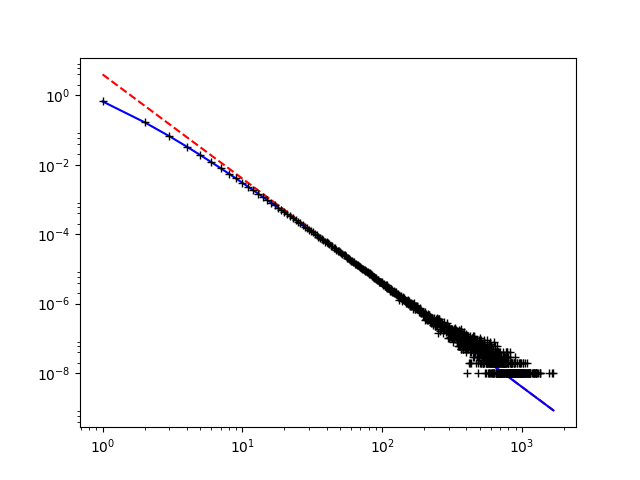
\includegraphics[width=\textwidth]{Datafit-m=1N=5.png}
 			\caption{$m=1$}
 		\end{subfigure}%
 		\begin{subfigure}{.6\textwidth}
 			\centering 
			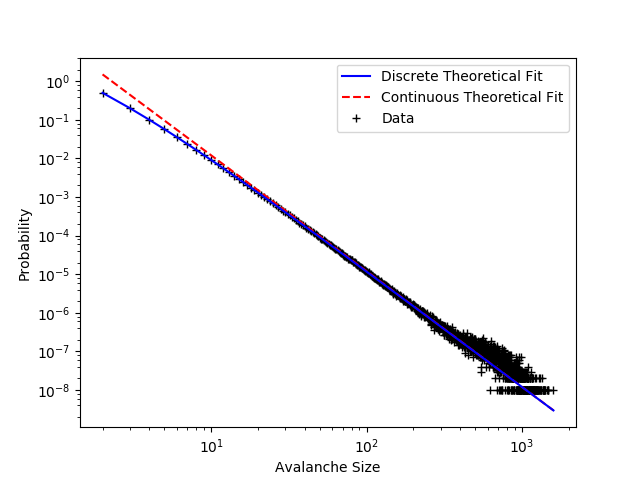
\includegraphics[width=\textwidth]{Datafit-m=2N=5.png}
 			\caption{$m=2$}
 		\end{subfigure}
 	}
 		\baselineskip
 	\makebox[\linewidth][c]{%
 		\begin{subfigure}{.6\textwidth}
 			\centering 
		 	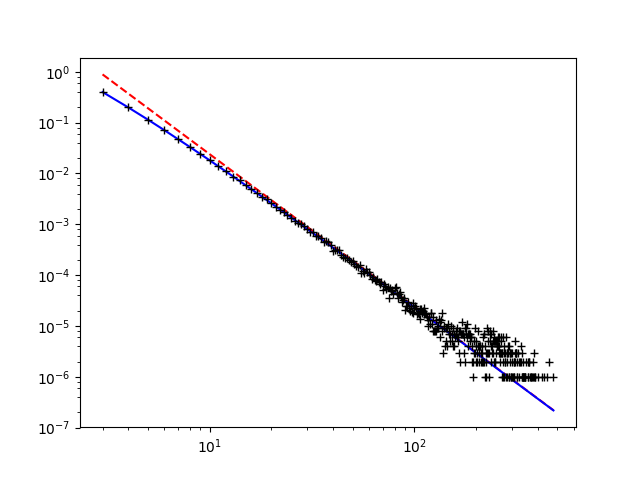
\includegraphics[width=\textwidth]{Datafit-m=3N=5.png}
 			\caption{$m=3$}
 		\end{subfigure}%
  		\begin{subfigure}{.6\textwidth}
  			\centering 
  			\includegraphics[width=\textwidth]{Datafit-m=4N=5.png}
  			\caption{$m=4$}
  		\end{subfigure}
 	}
 	\caption{The loglog plots of the raw data porbability distribuiton. This data was captured from networks of size $10^5$, and over $10^3$ traisl. a,b,c,d show the outcome for m=1,2,3,4 repectively.}
\end{figure}
 Figure 4 shows the continuous and discrete fits derived earlier. Visually, one can see from that for small values of $k$, the probability distribution follows the discrete fit perfectly. This is because there are a lot more nodes with degree small $k$, and so a lot more data is available, thus the distribution is prominent. However, for large $k$ we have fewer and fewar nodes per degree, as predicted. This creates the 'fat tail' affect present on all three figures as seen in . \\
Notice as well that as m increase, our theoretical, and practical data moves closer to the line $p(k)=k^{-3}$. This verifies the effect I would expect to see for large m.
\subsection{Statistical Approach}
I wish to analyse the model statistically. However, the 'fat tail' characteristic of the data means that the majority of our points lie near the origin. Therefore any statistical method I use will be dominated by the 'fat tail', and any conclusion I draw will be obscured. Log binning is way of mimising the 'fat tail, while keeping the necessary characteristics of the probability distribution.\\
When creating probability distributions from samples, data is put into bins, the frequency recorded and then normalised. In most cases we have a bin lengths constant, $b_{n+1}-b_{n}=:\Delta$. However in a log bin proccess, the bins have a relation $\frac{b_{n+1}}{b_n}=\Delta$. This means that the bins increase exponentially as the data grows larger. \\
This means for small $k$, where the data are plentiful, the bins are small to capture as much information as possible. However for large $k$,  where our data is sparse, the bins are large, meaning the a lot of data is grouped together to help gain insight into the behviour. The geometric mean of each bin is then plotted. Figure 4 shows how the log bin processes the raw data.

\begin{figure}[htbp]
	\centering
	%\includegraphics{figure_1.png}
	
	\includegraphics[width=.7\textwidth]{LogBin.png}
	\caption{The degree distribution for random attachment. Note the distinctive exponential cut off and lack of a fat tail. This data was taken from graphs of N=10,000, over 100 trails, for m=1,2,3,4.}
\end{figure}	 	
 
To statistically analyse this data I plotted the theoretical fit and naive fit vs. the actual logbinned data. Assuming that my two fits and the actuall data are related, one would expect to see a linear regression between the variables. Figure 5 shows an example of this.
\begin{figure}[H]
	 	 	\makebox[\linewidth][c]{%
	 	 		\begin{subfigure}{.5\textwidth}
	 	 			\centering 
	 	 			\includegraphics[width=\textwidth]{LR-m=4LB.png}
	 	 		\end{subfigure}%
	\begin{tabular}{l|l|l|l|l|l|l|}
		\cline{2-7}
		& \multicolumn{6}{l|}{Linear Regression for Log Binned Data}            \\ \cline{2-7} 
		& \multicolumn{3}{l|}{Naive Fit} & \multicolumn{3}{l|}{Theoretical Fit} \\ \cline{2-7} 
		& $R^2$   & p-value    & Slope   & $R^2$     & p-vaule      & Slope     \\ \hline
		\multicolumn{1}{|l|}{m=1} & 0.992   & 2.71e-25   & 0.1628  & 0.999     & 2.87e-40     & 0.9824    \\ \hline
		\multicolumn{1}{|l|}{m=2} & 0.993   & 2.71e-25   & 0.3637  & 0.999     & 2.86e-40     & 1.0444    \\ \hline
		\multicolumn{1}{|l|}{m=3} & 0.993   & 2.72e-25   & 0.4886  & 0.996     & 2.69e-28     & 1.0394    \\ \hline
		\multicolumn{1}{|l|}{m=4} & 0.991   & 2.35e-24   & 0.5719  & 0.994     & 2.72e-26     & 1.0312    \\ \hline
	\end{tabular}%
	 	 		
	 	 	}
	 	 	
	 	   		\caption{The theoretical model(red) and the naive model(black) vs. the log binned, for $m=4$.
	 	   			}
\end{figure}
 These relation can be explored further by calculating the least squares regression statistics($R^2$). I used the Pearson $R^2$ statistic as the visual evidence from figrue 5 implies that our relation is linear. Using these I tested with the null hypothesis that there is no correlation vs. the hypothesis that they are correlated. The $R^2$ statistic, the p-values for this hypotesis, and the least regression slope can be found in figure 5b).\\

The p-statistic is very small in all cases. Infact we can reject the null hypothesis with a confidence level of 1.e-25 for each fit. This impies that there is definitly correlation, and therefore both models would suffice.\\
To analyse which model is better one needs to examine the $R^2$ terms and slopes. For all $m$, the $R^2$ statistic is greater for the theoretical fit, than that of the naive fit. This implies that the theoretical fit is better.\\
Analysing the slope, one would expect the slope to be close to 1, if the theoretical explained the actual data well. Refering to figure b) shows that is is true for the theoretical fit. \\
Note that the difference $R^2$ statistics for the two fits shrinks. This is more evidence that points towards the phenomena that as m increases our two fits converge.    
\section{Finite Size Effect}
\subsection{Theoretical Derivation}
I wish to find how the greatest degree $k_1$. First I assume that there is only one node with degree $k_1$. And therefore:
\begin{equation}
\sum_{k1}^{\infty} p_{\infty}(k)=\frac{1}{N(t)}
\end{equation}
From the partial fraction form of the degree distribution, and applying the same logic as I did for normalisation, we have
\begin{equation}
\sum_{k_1}^{\infty}	\frac{2m(m+1)}{k(k+1)(k+2)}=\frac{2m(m+1)}{2k_1(k_1+1)}=\frac{1}{N(t)}
\end{equation}
Rearranging this formula gives a quadratic in $k_1$,
\begin{equation}
	2k_1(k_1+1)=2Nm(m+1) \Rightarrow k_{1}^{2} + k_1 -Nm(m+1)=0
\end{equation}
The positive solution gives,
\begin{equation}
	k_1 = \frac{1}{2}(-1 + \sqrt{1+4Nm(m+1)})
\end{equation}
Therefore, for large N and m, we expect, $k_1 \propto \sqrt{N}$ . 
\subsection{Experimental Data}
To test how $k_1$ scales $N$, I ran my program for $N=10^2, 10^3, 10^4, 10^5$, collecting the maximum degrees. I focus on $m=4$, the maximum $m$ I recorded. This is because I need to fulfill the  $Nm>>1$ condition in order to observe $k_1 \propto \sqrt{N}$. We are interested in these larger degrees, as they obviously depend a lot more on the finite size of the graph. The fact that this is an extreme statistic means that it is very intermittent, and therefore one would expect to see a lot of variance between trials. Therefore I repeated this experiment 100 times, taking the mean and variance to gain a better statistic. 
\begin{figure}[H]
	\makebox[\linewidth][c]{%
		\begin{subfigure}{.6\textwidth}
			\centering
			\includegraphics[width=\textwidth]{k1.png}
			\caption{}
		\end{subfigure}%
		\begin{subfigure}{.6\textwidth}
			\centering 
			\includegraphics[width=\textwidth]{k1Log.png}
			\caption{}
		\end{subfigure}
	}
	\caption{The mean $k_1$ for $N=10^2, 10^3, 10^4, 10^5$. The fit(red line) is the one described by equation (20). a) Shows the plot, and b) shows the log-log plot.}
\end{figure}
Figure 6 (a) shows that the fit my not entirely describe the dependence of $k_1$, however in figure 6 (b), the fit and the data are parallel, in log space. This implies that  $k_1$ does scale with $\sqrt{N}$.
\subsection{Data Collapse}
Since we now know how the degree distribution depends on $k$, $m$ and $N$, I can perform a data collapse. I concentrate on m=4, as it gives me better statistical data for large degree sizes. I vary $N=10^2, 10^3, 10^4, 10^5$. Figure 6 shows a plot of how the uncollapsed degree distributions correlate. 
\begin{figure}[H]
		\makebox[\linewidth][c]{%
			\begin{subfigure}{.6\textwidth}
				\centering
				\includegraphics[width=\textwidth]{Collapse11.png}
				\caption{}
			\end{subfigure}%
			\begin{subfigure}{.6\textwidth}
				\centering 
				\includegraphics[width=\textwidth]{Collapse2.png}
				\caption{}
			\end{subfigure}
		}
		\baselineskip
		\makebox[\linewidth][c]{%
			\begin{subfigure}{.6\textwidth}
				\centering 
				\includegraphics[width=\textwidth]{Collapse1.png}
				\caption{$m=3$}
			\end{subfigure}%
		}
				\caption{a) Shows the uncollapsed probability distributions for $N=10^2,10^3,10^4,10^5$ , $m=4$. b) Shows the collapse when dividing through by the theoretical distribution.  }
\end{figure} 
First I collapse the probability distribution in k by dividing through by my theoretical prediction:
\begin{equation}
	c_k(N)=\frac{p_{data}(k)}{p_{theory}(k)}
\end{equation}
Figure 5 shows the outcome of this proccedure.
Now I collapse in N. To do this I use the relation I earlier derived of how the $k_1$ scales with $N$. I stretched the degrees observed by a factor of $N^{-\frac{1}{2}}$. Figure 7 shows the full collapse.\\
In both cases, instead of using errorbars, I have opted to just plot the raw data to show the spread of the data. For a single trail, this is not good measure, as extreme statistics are few and far between. However over a large number of trails (1000 in this case), the structure of the data becomes very apparent. For $N=10^5$ one can see that there are still a few outlying points, implying that more trail maybe necessary to get an exact idea of the spread, however I still feel the behaviour of the data is still captured fairly well.
\section{Random Attachement}
It is also useful, to see how preferential attachment compares with a graph with random attachment. In this network has the same probability of being having an edge attached, or mathematically $\Pi(k,t) = \frac{1}{N(t)}$, where $N(t)$ normalizes the probability.
\subsection{Degree Distribution}
The master equation will be the same as when considering preferential attachment. 
\begin{equation}
n(k,t+1)=n(k,t)+m\Pi(k-1,t)n(k-1,t)-m\Pi(k,t)n(k,t)+\delta_{k,m}
\end{equation}
Using the new probabilities and that $p(k,t)=n(k,t)/N(t)$:
\begin{equation}
N(k,t+1)p(k,t+1)-N(k,t)p(k,t)=mp(k-1,t)-mp(k,t)+\delta_{k,m}
\end{equation}
Assuming that $\lim\limits_{t \rightarrow \infty} p(k,t)=p_\infty(k)$:
\begin{equation}
p_{\infty}(k)= mp_{\infty}(k-1)-mp_{\infty}(k) + \delta_{k,m}
\end{equation}
Concentrating on the case $k=m$:
\begin{equation}
p_{\infty}(m)= -mp_{\infty}(m) + 1 \quad
\Rightarrow \quad p_{\infty}(m)= \frac{1}{m+1}
\end{equation}
Using this probability to the case k=m+1:
\begin{equation}
p_{\infty}(m+1)= \frac{m}{m+1}-mp_{\infty}(m+1)
\quad\Rightarrow\quad p_{\infty}(m+1)= \frac{m}{(m+1)^2}
\end{equation}
Therefore I make the assumption that $p_{\infty}(k)= (\frac{1}{m+1})(\frac{m}{m+1})^{k-m}$ it true for all $k$. Using the case $k=m$ as an anchor step, and proving the relation from $k>m$ and $k+1$:
\begin{equation}
\begin{align}
&p_{\infty}(k+1)= mp_{\infty}(k)-mp_{\infty}(k+1)\\
&\Rightarrow p_{\infty}(k+1)= m\left(\frac{1}{m+1}\right)\left(\frac{m}{m+1}\right)^{k-m}-mp_{\infty}(k+1)\\
&\Rightarrow p_{\infty}(k+1)=\left(\frac{1}{m+1}\right)\left(\frac{m}{m+1}\right)^{(k+1)-m}
\end{align}
\end{equation}
Therefore by induction the above assumption is true. To check that this equation is normalised:
\begin{equation}
\begin{align}
	&\sum_{k=m}^{\infty}p_{\infty}(k)= \
	\left(\frac{1}{m+1}\right)\sum_{k=m}^{\infty}\left(\frac{m}{m+1}\right)^{k-m}\\
	&\Rightarrow = \left(\frac{1}{m+1}\right)\left(\frac{m+1}{m}\right)^{m}\sum_{k=m}^{\infty}\left(\frac{m}{m+1}\right)^{k}\\
&\Rightarrow \left(\frac{1}{m+1}\right)\left(\frac{m+1}{m}\right)^{m}\left( \frac{\left(\frac{m}{m+1}\right)^m}{1-\frac{m}{m+1}}\right) =1
\end{align}
\end{equation}
The numerical degree distribution for the random attachment follows the theoretical distributions derived(figure ..4..). Unlike the preferential attachment, the random data does not have a fat tail, and appears to follow and exponential cut-off instead. This is to be expected, as it is a lot less likely to find big hubs in a this model, than that of preferential attachment. This implies that this model is does not follow a power law and is therefore not a scale free network. 
\begin{figure}[htbp]
	\centering
	%\includegraphics{figure_1.png}
	
	\includegraphics[width=.7\textwidth]{RandomGraph1.png}
	\caption{The degree distribution for random attachment. Note the distinctive exponential cut off and lack of a fat tail. This data was taken from graphs of N=100,000, over 100 trails, for m=1,2,3,4.}
\end{figure}
\subsection{Theoretical Derviation of Largest Degree}
Using the same logic as with the preferential largest degree,
\begin{equation}
\left(\frac{1}{m+1}\right) \sum_{k_1}^{\infty} \left(\frac{m}{m+1}\right)^{k-m} = \frac{1}{N}
\end{equation}
Changing the index to $k=k_1 + k'$, we have,
\begin{equation}
	\left(\frac{m}{m+1}\right)^{k_1-m} \sum_{k'=0}^{\infty} \left(\frac{m}{m+1}\right)^{k'} = \frac{m+1}{N}
\end{equation}
It is obvious that $\left| \frac{m}{m+1} \right| < 1$, and so we can treat it as a convergent geometric sum:
\begin{equation}
\begin{align}
&\left(\frac{1}{m+1}\right)^{k_1-m} \left(\frac{m}{1-\frac{m}{m+1}}\right) = \frac{m+1}{N}\\
&\Rightarrow \left(\frac{m}{m+1}\right)^{k_1-m} (m+1)= \frac{m+1}{N}\\
&\Rightarrow \left(\frac{m}{m+1}\right)^{k_1}= \frac{m^m}{N(m+1)^m}
\end{align}
\end{equation}
Taking the logarithm,
\begin{equation}
\begin{align}
&k_1 \log\left(\frac{m}{m+1}\right)= m\log\left(\frac{m}{m+1}\right) -\log(N)\\
&k_1 = m -\frac{\log(N)}{\log(m)-\log(m+1)}
\end{align}
\end{equation}
Therefore we have that $k_1 \propto log(N)$ for large $N$. Note that $k_1$ does not follow a power law relation with growth, implying again that this is not a scale-free network. \\
\begin{figure}[htbp]
	\centering
	%\includegraphics{figure_1.png}
	
	\includegraphics[width=.7\textwidth]{k1random.png}
	\caption{The mean largest degree $k_1$ of the random attachment model. The data was taken from 100 trials, for $m=4$, $N=10^2, 10^3, 10^4, 10^5$. Error bars represent the standard deviation of each sample. The blue line is the theoretical fit desribed in (35). This data follows this fit to a high level of accuracy. }
\end{figure}
\section{Random Walk Preferential Attachment}
This case is similar to that of the random attachment, however every vertex we pick, we then perform a random walk of length L, and attach an edge to our finishing node. I will study the behaviour of this model for different walk size L. 
\subsection{$L=0$}
This case is trivial. If L=0, then we do not perform a random walk, and we recover the random preferential attachment case from before.
\subsection{$L=1$}
This case is more interesting. Figure 11 (a) shows the degree distributions for $m=1,2, 10$. One can see that fat tails are present and that the distributions do follow a power law,  implying it is a scale-free network. However, unlike the BA model, the power law is dependent on $m$, the number of edges added per timestep. \\
The algorithm used is very similar to that of the mediation-driven attachment networks(MDA)(Figure 11 (b)). The MDA model uses preferential attachment like the BA. However, for small m, instead of being desrcibed as using the \textit{'rich-get-richer'} mechanism like the BA, it is often described as using the \textit{'winners take it all'} mechanism, i.e. there are even fewer, more connected hubs. \\
These networks are created using an almost identical to our algoirthm. The only difference being that, one chooses a single random vertex and chooses from that node's neighbourhood m times, instead of choosing m random vertices and choosing once from each neighbourhood. These networks have been shown to exhibit a power law relation $P(k,m) \~ k^{-\gamma(m)}$ where $\gamma= \frac{1}{\beta(m)}+1$ is a function of m[2]. Looking at the numerical data, I propose that the model for L=1 follows a similar relation.\\
\begin{figure}[H]
	\makebox[\linewidth][c]{%
		\begin{subfigure}{.6\textwidth}
			\centering
			\includegraphics[width=\textwidth]{RandomwalkL=1.png}
			\caption{}
		\end{subfigure}%
		\begin{subfigure}{.6\textwidth}
			\centering 
			\includegraphics[width=\textwidth]{MDA.png}
			\caption{}
		\end{subfigure}
	} 
	\caption{(a) Shows the model for L=1, $m=1,2,10$ and $N=10,000$, over 100 trials. (b) Shows the MDA model for the same parameters. There is some difference between the two models, especialy for $m$ and $k$. However, with $m=1,2$, both models  exhibit the 'Winners take it all' behaviour for small m. I.e. The $p(m) \approx 1$, so the majority of the nodes in our network have minimum degree, with a few small 'super hubs' with large degree.\\
		Also note that the gradient of the log log plot in both cases increase with m. This implies that with have a power law dependent on $m$ as suggested.}
\end{figure}
\subsection{$L > 1$}
To explore how the graph changes with longer random walks, I chose 4 cases for L. 
\begin{enumerate}
	\item L=2, to understand what happens for L close to 1.
	\item L=4, as the shortest path from a node tot he node with maximum degree is $<l> \sim \frac{\log(N)}{\log(\log(N))} \approx 4$, for N=10,000[3]. 
	\item L=9, As the diameter in the BA model is $D \sim \log(N) \approx 9 $ for N=10,000[3].
	\item L=100 to reveal the behaviour distribution as $L >>1$.
\end{enumerate}
\begin{figure}[H]
			\makebox[\linewidth][c]{%
				\begin{subfigure}{.6\textwidth}
				\centering				\includegraphics[width=\textwidth]{Theoretical4.png}		
	\caption{}
			\end{subfigure}%
			\begin{subfigure}{.6\textwidth}
				\centering 					
				\includegraphics[width=\textwidth]{Theoretical6.png}
				\caption{}
			\end{subfigure}
			} 
			\caption{a) shows the degree distribution for $N=10^4$, $m=1$, captured over 100 trials, $L=2,4,100$. As L increases there is slight evidence of convergence towards the theoretical fit of BA model, although, all three cases obviously shows behaviour similar to preferential attachment.\\
			(b) Shows the curious case one when L is the diameter of the graph. For this data was captured over 100 trials, from $N=10^3,10^4,10^5$, and $L=7,9,11$ (diameters for respecting network size). Unlike other cases, the degree distribution does not appear to follow the fit, however appears to follow an almost exact, different, power law. The example above(black line) is $p_{\infty}(k) \propto k^{-2.5}$. Another interesting feature, is the size of the fat tail. Lookng at $N=10^4$, the fat tail for $L=9$ is roughly 15 times larger than that of $L=100$.  }	
\end{figure}
As figure 12a) shows, there is large change in the degree distribution for $L>1$. An interesting feature is that we also recover the BA model. A possible reason for this could be that by performing large walks, we actually recover the noton of eigenvalue centrality. I.e. the probability of landing on a specific node is proportional to it's centrality in the network, and so central nodes are more likely to picked, recovering preferential attachment. This idea is used in analysis methods such as broadcasting and diffusion processes. \\
Figure 12b) shows and describes the curios phenomenon of the third case, when $L \approx D$. In the future I wish to study this case in more detail, to understand why this feature occurs both mathematically and physically.\\


[2]Degree distribution, rank-size distribution, and leadership persistence in mediation-driven attachment networks, chapter 4, page 27. Kamrul Hassan et al.
[3]Structural Properties of Scale-Free Networks, chapter 4.2.3, page 10. Reuven Cohen et al.




\end{document}
